\subsubsection{Как обеспечить стабильность положение РТ в каскаде на УПТ?}

УПТ с управляющим p-n-переходом, изменение температуры приводит к:\\
1) изменению разности потенциалов на p-n-переходе;\\
2) изменению обратного тока на нём;\\
3) изменению $\mu_{n}$,$\mu_{p}$ (подвижные носители);\\
При увеличении температуры $\varphi_{k}$ уменьшается [$\varphi_{T}=\frac{kT}{q}$], следовательно сопротивление управляемого перехода уменьшается, увеличивается напряжение отсечки, следовательно увеличивается ток через канал.\\
При увеличению температуры $\mu_{n}$,$\mu_{p}$ уменьшаются, следовательно сопротивление канала увеличивается, ток канала уменьшается.
Эти процессы скомпенсируются и ток в канале не будет зависеть от температуры. Точка на ВАХ (стоко-затв.), в которой $I_{kanal}\ne f(T)$, - термостаб. точка.
\begin{center}
\begin{figure}[h!]
\center{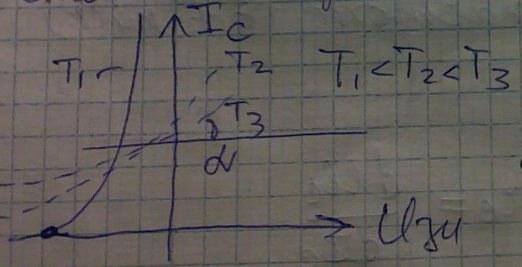
\includegraphics[scale=0.7]{p3_24.png}}
\end{figure}
\end{center}
Крутизна ВАХ уменьшается, следовательно $K_{U}$общ. уменьшается.\\
Для стабилизации РТ в таком каскаде используется ООС по току:
\begin{center}
\begin{figure}[h!]
\center{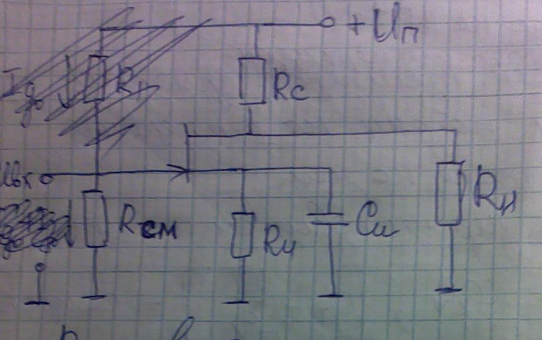
\includegraphics[scale=0.7]{p3_24(2).png}}
\end{figure}
\end{center}

$R_{\text{см}}$ выбирается меньше $R_{in}$
\begin{center}
\begin{figure}[h!]
\center{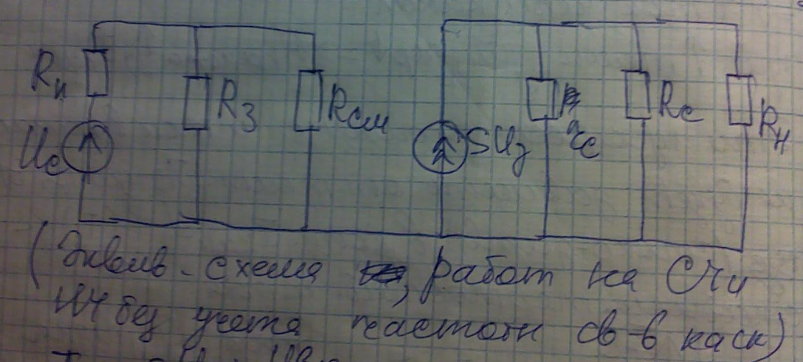
\includegraphics[scale=0.7]{p3_24(3).png}}
\end{figure}
\end{center}

$I_{c}=SU_{\text{з}}+\frac{U_{out}}{r_{c}}$\\
$r_{c}$ - дифф сопротивление, $r_{c}=\frac{dU_{c}}{dI_{c}}$\\
$$
U_{out}=I_{c}R_{c}=R_{c}(SU_{\text{з}}+\frac{U_{out}}{r_{c}})
$$
$$
U_{out}(\frac{r_{c}-R_{c}}{r_{c}*R_{c}})=SU_{\text{з}}
$$
$$
K_{U}=\frac{U_{out}}{U_{\text{з}}}=\frac{S*R_{c}*r_{c}}{r_{c}-R_{c}}
$$
(сигнал инвертируется, следовательно отриц.)\\
$r_{c}>>R_{c}$ следовательно $K_{U}\approx SR_{c}$
$$
R_{in}=\frac{R_{\text{см}}R_{\text{з}}}{R_{\text{см}}+R_{\text{з}}}\approx R_{\text{см}}
$$
$R_{\text{з}}\approx 1MOm$
$$
R_{out}=\frac{R_{c}r_{c}}{r_{c}+R_{c}}\approx R_{c}
$$
Для ООС:
$$
\beta=\frac{U_{out\text{ЦОС}}}{U_{in\text{ЦОС}}}=\frac{U_{OC}}{U_{out}}=\frac{I_{c}R_{u}}{I_{c}R_{c}}=\frac{R_{u}}{R_{c}}
$$
Отрицательная ОС:
$$
K_{UOS}=\frac{K_{U}}{1+\beta*K_{U}}=\frac{SR_{c}}{1+SR_{c}*\frac{R_{U}}{R_{c}}}=\frac{SR_{c}}{1+SR_{U}}
$$
Следовательно глубина ОС равна $1+SR_{U}$\\
Следовательно: $\Delta I_{c_{0}OOC}=\frac{\Delta I_{c_{0}}}{1+SR_{U}}$\\
Определение значения $R_{u}$:\\
на стоко-затворной ВАХ выбирается точка ($U_{\text{зн}_{0}}$,$I_{\text{с}_{0}}$)\\
$I_{\text{з}_{0}}\approx 0$ следовательно $U_{\text{см}_{0}}= 0$ следовательно $R_{u}=\frac{U_{\text{зн}_{0}}}{I_{\text{с}_{0}}}$
\begin{center}
\begin{figure}[h!]
\center{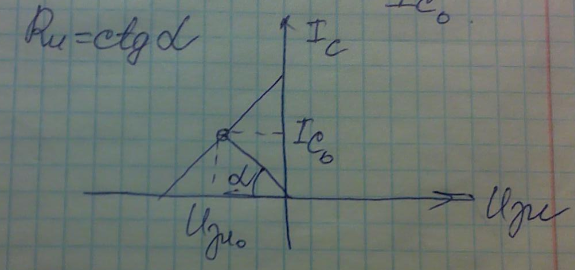
\includegraphics[scale=0.7]{p3_24(4).png}}
\end{figure}
\end{center}
